\documentclass[red]{beamer}


\mode<presentation> {
  \usetheme{Warsaw}
  \setbeamercovered{transparent}
}


\usepackage{beamerthemesplit} 
\usepackage[czech]{babel}
\usepackage[utf8]{inputenc}
\usepackage[T1]{fontenc}
\usepackage{listings}

\title{Distribuovaný systém kontroly verzií - Git}    
\author{Juraj Hreško}                 
\institute{ecommerce.cz}      
\date{\today}                 

\begin{document}

\begin{frame}
  \titlepage
\end{frame}


\section{Verzovacie systémy} % 1. Kapitola



\begin{frame}
  \frametitle{Požiadavky na SCM}   
  \begin{itemize}
  \item ukladanie dát do archívu (repozitára)

  \item obnovenie dát z určitej doby

  \item porovnávanie verzií dát

  \item anotovanie dát

  \item riešenie prítupu viacerých vývojárov

 \item označovanie verzií špecifickým menom

 \item vetvenie vývoja

 \item zlučovanie vetví vývoja
  \end{itemize}
\end{frame}

\begin{frame}
  \frametitle{Typy verzovacích systémov}   
  \begin{itemize}
  \item "triviálne"
  \item centralizované (client-server)
  \item distribuované
  \end{itemize}
\end{frame}

\begin{frame}[fragile]
  \frametitle{"Triviálne"  verzovanie}   
   
  Použil už snáď každý pri zálohe napr. konfiguračných súborov. 

\begin{block}{Príklad}
\begin{verbatim}
    $ cp config.cfg config.old
    c:\>copy config.cfg config.old
\end{verbatim}
\end{block}

\begin{itemize}
\item vhodné pre jednu dostupnú "zálohu"
\item nesystematické pre viac súborov s históriou
\item nehovoriac o zdieľaní, vetvení a pod.
\end{itemize}

\end{frame}

\begin{frame}
  \frametitle{Centralizované systémy pre správu verzií}   

\begin{itemize}
\item architektúra typu klient-server
\item spoločný centrálny repozitár
\item vývoj prebieha v rámci pracovnej kópie
\item riešenie súčasného zápisu viacerých programátorov
\begin{itemize}
\item lock/modify/commit
\item modify/merge/commit
 \end{itemize}
\item zástupcovia: CVS, SVN, Perforce, TFS
 \end{itemize}
\end{frame}

\begin{frame}
  \frametitle{Distribuované systémy pre správu verzií}   

\begin{itemize}
\item neexistuje centrálny repozitár - každý je plnohodnotný
\item miesto operácie checkout operácia clone
\item repozitár == pracovná kópia
\item publikovanie zmien - vystavenie repozitára, push do vzdialenej vetvy, posielanie záplat e-mailom
\item zástupcovia: Monotone, Git, Mercurial, Bazaar
 \end{itemize}
\end{frame}

\section{Výhody DSCM (Git)} % 2. Kapitola

\begin{frame}
  \frametitle{Práca s lokálnym repozitárom}   

\begin{itemize}
\item neexistuje "jedno zraniteľné miesto" (single point of failure)
\item offline práca s repozitárom (vo vlaku, na chate, pri výpadku serverov)
\begin{itemize}
\item prechádzanie histórie
\item commity
\item vetvenie
 \end{itemize}
\item súkromie pri experimentoch
\item rýchlosť operácií
 \end{itemize}
\end{frame}

\begin{frame}
  \frametitle{Práca s repozitármi - schéma}

  \begin{figure}
  \centering
  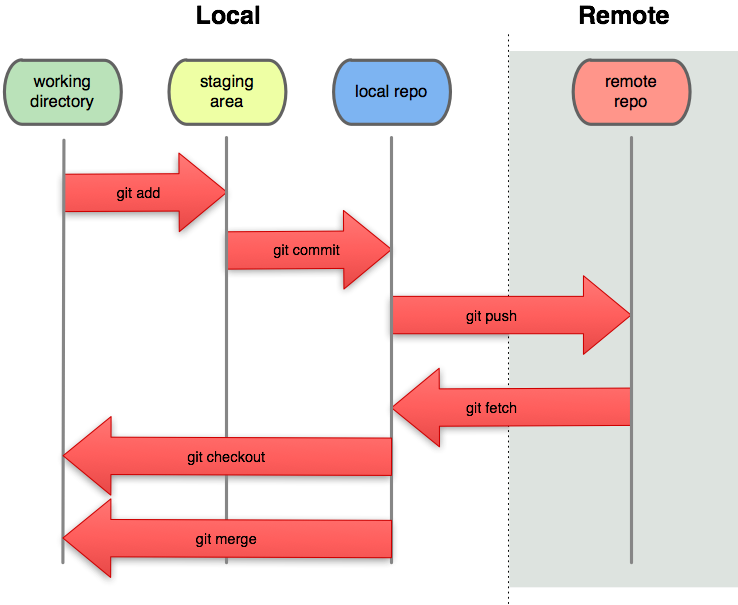
\includegraphics[scale=0.7]{git-pics/local-remote.png}
\end{figure}
\end{frame}

\subsection{Flexibilný workflow}
\begin{frame}
\frametitle{Flexibilný workflow}
\begin{itemize}
\item je možné pracovať s repozitármi rôznymi spôsobmi, v závislosti od druhu projektu
\item iné pre klasický centralizovaný vývoj, vlastné dokumenty, vývoj open source software
\item príklady niektorých možných workflow
\begin{itemize}
\item centralizovaný 
\item koordinátor
\item generál a pobočníci
 \end{itemize}
 \end{itemize}
\end{frame}

\begin{frame}
  \frametitle{Centralizovaný workflow}

  \begin{figure}
  \centering
  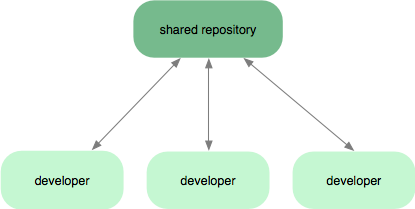
\includegraphics[scale=1]{git-pics/workflow-a.png}
\end{figure}
\end{frame}

\begin{frame}
  \frametitle{Workflow "koordinátor"}

  \begin{figure}
  \centering
  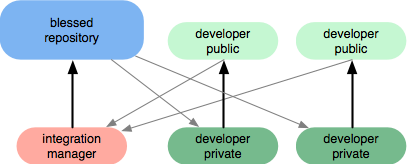
\includegraphics[scale=1]{git-pics/workflow-b.png}
\end{figure}
\end{frame}

\begin{frame}
  \frametitle{Workflow "generál a pobočníci"}

  \begin{figure}
  \centering
  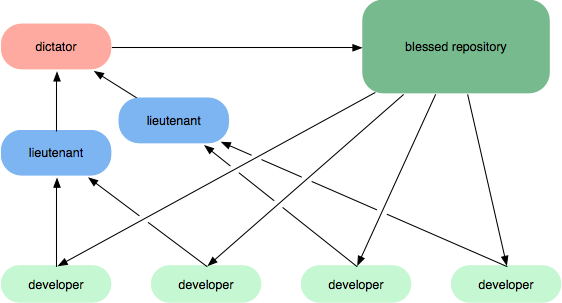
\includegraphics[scale=1]{git-pics/workflow-c.png}
\end{figure}
\end{frame}

\section{Git} % 3. Kapitola	

\subsection{Na úvod ku Gitu}
\begin{frame}
\frametitle{Krátko k histórii projektu}

\textbf{ git \\
 \textit{1.	a contemptible person, often a fool\\
2.	a bastard}} \\ 
\textbf{ \tiny{ (Collins English Dictionary)}}
\begin{itemize}
\item vznik v roku 2005, k účelu verzovania projektu linuxového jadra
\item hlavné požiadavky 
\begin{itemize}
\item Take CVS as an example of what not to do; if in doubt, make the exact opposite decision
\item Support a distributed, BitKeeper-like workflow
\item Very strong safeguards against corruption, either accidental or malicious
\item Very high performance
 \end{itemize}
\item spočiatku sada programov v Perl, Bash a C
 \end{itemize}
\end{frame}

\begin{frame}
  \frametitle{Súčasnosť projektu}   

\begin{itemize}
\item voľne dostupný open source DSCM software
\item stránky projektu \href{http://git-scm.com/}{http://git-scm.com/}
\item používaný aj na väčších projektoch
\begin{itemize}
\item Git
\item Linux Kernel
\item Android
\item Ruby on Rails
\item Fedora
\item VLC media player
\item \dots
 \end{itemize}
\item primárne pre platformu GNU/Linux a ostatné Unix-like systémy - BSD, Solaris, Darwin
\item pre MS Windows v Cygwin alebo port mysysgit
\item základom je ovládanie cez príkazový riadok, dostupné však aj GUI a pluginy pre IDE (Eclipse, NetBeans, Visual Studio)
 \end{itemize}
\end{frame}

\subsection{Práca s Gitom}

\begin{frame}[fragile]
\frametitle{Inštalácia}   

Pre GNU/Linux  balíček v repozitári - git-core
\begin{block}{Príklad}
\begin{verbatim}
$ yum install git-core		
$ apt-get install git-core		
\end{verbatim}
\end{block}
Pre MS Windows doporučujem kombináciu msysgit + TortoiseGit
\begin{itemize}
\item \href{http://code.google.com/p/msysgit/}{msysgit} - posledná verzia \href{ http://code.google.com/p/msysgit/downloads/detail?name=Git-1.7.2.3-preview20100911.exe}{Git 1.7.2.3}
\item pri výbere komponent doporučujem zrušiť Windows Explorer integration (zabezpečí ho TortoiseGit)
\item ostatné voľby podľa uváženia, osobne ponechávam východzie
\item následne doinštalovať GUI klienta - \href{ http://code.google.com/p/tortoisegit/}{TortoiseGit}
\item pri inštalácii je dobré zvoliť totožného SSH klienta ako u Gitu, v mojom prípade u oboch OpenSSH
 \end{itemize}
\end{frame}

\begin{frame}[fragile]
\frametitle{Veľmi stručný úvod k použitiu (Git) Bash}   
Git Bash spustíme, z menu Programy/Git/Git Bash. Práca v Bash konzoli je podobná práci s príkazovým riadkom vo Windows/DOS. 
Niekoľko základných príkazov:
\\
\begin{tabular}{|l||l|l|}

\hline
  {\bf Bash} & {\bf cmd.exe} &  {\bf Popis} \\
\hline
\hline
  cd & cd   &  Zmení adresár  \\
  cp & copy  & Skopíruje súbor(y) \\
  rm & del  & Zmaže súbor(y) \\
  mkdir & mkdir & Vytvorí adresár \\
  ls & dir & Vypíše obsah adresáru \\
  cd /c & c: & Zmení adresár na koreň disku C: \\
\hline
\end{tabular}
\\ 
Text zo schránky vkladáme pomocou Shift+Insert.
Podrobná nápoveda k príkazu - parameter - - help
\begin{block}{}
\begin{verbatim}
$ mkdir --help	
\end{verbatim}
\end{block}
\end{frame}

\begin{frame}[fragile]
\frametitle{Založenie repozitára}   
V ľubovoľnom existujúcom adresári zadáme príkaz \texttt{git init}

\begin{block}{}
\begin{verbatim}
$ cd /c
$ mkdir git-workshop
$ mkdir testproject
$ cd git-workshop/testproject
$ git init
Initialized empty Git repository in c:/git-workshop/testprojekt/.git/	
\end{verbatim}
\end{block}

Po tomto kroku môžeme začať verzovať ľubovoľné súbory a adresáre, ktoré sa nachádzajú v adresári \texttt{testrepo}.
\end{frame}

\begin{frame}[fragile]
\frametitle{Pred prvým commitom}   

Po inštalácii Gitu je dobré nastaviť do konfigurácie správne údaje o autorovi.

\begin{block}{}
\begin{verbatim}
$ git config --global user.name "Michal Muthsam"
$ git config --global user.email muthsam@ecommerce.cz
\end{verbatim}
\end{block}
Ďalej si pripravíme nejaký súbor, ktorý budeme v ďalšom kroku verzovať. Vytvoríme napríklad textový súbor ahoj.txt a vložíme do neho nejaký text. Toto môžeme spraviť v Notepade (prípadne inom editore), alebo priamo z konzole.
\begin{block}{}
\begin{verbatim}
$ cd /c/testproject
$ touch ahoj.txt
$ echo Nazdar svet! > ahoj.txt
\end{verbatim}
\end{block}
\end{frame}

\begin{frame}[fragile]
\frametitle{Náš prvý commit}   

\begin{columns}
\begin{column}[l]{7cm}
Máme pripravený súbor a radi by sme ho pridali do repozitára. Najskôr označíme zmeny, ktoré chceme zahrnúť do commitu, v tomto prípade súbor ahoj.txt, pomocou príkazu git add. \\
Potom použijeme git commit, s parametrom -m, ktorým pridáme popis commitu.
\end{column}
\begin{column}[r]{5cm}
\begin{figure}
  \centering
  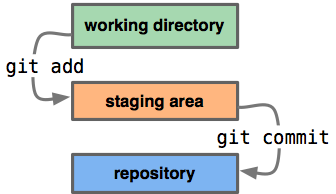
\includegraphics[scale=0.9]{git-pics/staging1.png}
\end{figure}
\end{column}
\end{columns} 
\begin{block}{}
\begin{verbatim}
$ git add ahoj.txt
$ git commit -m "Prvy commit do repa"
[master (root-commit) deb7c00] Prvy commit do repa
 1 files changed, 1 insertions(+), 0 deletions(-)
 create mode 100644 ahoj.txt
\end{verbatim}
\end{block}
\end{frame}

\begin{frame}[fragile]
\frametitle{Commit "po starom"}   

\begin{columns}
\begin{column}[l]{7cm}
Samozrejme niekedy by sme uvítali automatický commit všetkých zmien, bez nutnosti ich označovania. K tomu to slúži parameter -a u príkazu git commit. 
\end{column}
\begin{column}[r]{5cm}
\begin{figure}
  \centering
  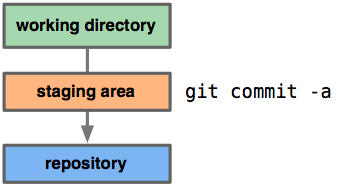
\includegraphics[scale=0.9]{git-pics/staging2.png}
\end{figure}
\end{column}
\end{columns} 
\begin{block}{}
\begin{verbatim}
$ echo Hello world! >> ahoj.txt
$ git commit -a -m "Pridany anglicky pozdrav"
[master 141d9c3] Pridany anglicky pozdrav
 1 files changed, 1 insertions(+), 0 deletions(-)
\end{verbatim}
\end{block}
\end{frame}

\begin{frame}[fragile]
\frametitle{Vytvorenie verejného repozitára}
Git umožňuje pripojenie na vzdialený repozitár prostredníctvom HTTP, SSH, vlastného GIT protokolu, prípadne priamo cez súborový systém. \\
Pre ilustráciu práce so vzdialeným repozitárom si vytvoríme takzvaný "bare" repozitár. Tento neobsahuje pracovnú kópiu a používa sa pre publikovanie zmien pre "okolitý svet". Niekedy sa používa aj označenie public repository. Pre jednoduchšie rozpoznanie je názov takéhoto repozitára doplnený príponou .git .

\begin{block}{}
\begin{verbatim}
$ cd /c/git-workshop
$ mkdir public_repos
$ cd public_repos
$ git clone --bare ../testproject
Cloning into bare repository testproject.git...
done.
\end{verbatim}
\end{block}
\end{frame}

\begin{frame}[fragile]
\frametitle{Pripojenie na existujúci repozitár}   
Git umožňuje pripojenie na vzdialený repozitár prostredníctvom HTTP, SSH, vlastného GIT protokolu, prípadne priamo cez súborový systém. \\
Aby sme nemuseli zadávať pri operáciách celú cestu k nášmu public repozitáru, pridáme si ho medzi tzv. remote.

\begin{block}{}
\begin{verbatim}
$ cd /c/git-workshop/testproject
$ git remote add origin ../public_repos/testproject.git/
$ git remote
origin
\end{verbatim}
\end{block}

Odteraz sa na náš public repozitár môžeme odkazovať pod menom "origin". Podobne je možné pridať viacero ďalších aliasov pre vzdialené repozitáre. Vśetky nastavené si zobrazíme príkazom git remote.

\end{frame}

\begin{frame}[fragile]
\frametitle{Odosielanie a sťahovanie zmien}   
Pre operácie so vzdialeným repozitárom slúžia (okrem iných) príkazy git push a git pull.\\
Na ukážku zmenu v repozitári testproject vypropagujeme do public repozitára testproject.git (origin).

\begin{block}{}
\begin{verbatim}
$ cd /c/git-workshop/testproject
$ sed -i 's/Nazdar/Ahojl/g' ahoj.txt 
$ git commit -a -m "zamena nazdar za ahoj"
[master 483f007] zamena nazdar za ahoj
 1 files changed, 1 insertions(+), 1 deletions(-)
$ git push origin master
Counting objects: 5, done.
...
To ../public_repos/testproject.git/
    141d9c3..483f007  mastes -> master
\end{verbatim}
\end{block}
\end{frame}

\end{document}
